\documentclass{article}
\usepackage{graphicx}
\usepackage{subcaption}
\usepackage{amsmath}
\usepackage{pgfplots}
\pgfplotsset{compat=1.18}
\usepackage[margin=25truemm]{geometry}

\title{CSCI2750 Homework 1}
\author{Wong Cheuk Yin 1155192671}
\date{\today}

\begin{document}
    \maketitle 
    \section{Problem 1}
    \subsection{Part (a)}
    \begin{tikzpicture}
    \begin{axis}[
        width=12cm,
        height=6cm,
        xlabel={$f / \text{Hz}$},
        ylabel={$G(f)$},
        axis lines=middle,
        axis line style={thick},
        xmin=0, xmax=1200,
        ymin=0, ymax=5,
        xtick={400,1000},
        xticklabels={$400$, $1000$},
        ytick={0,1,2,3,4},
        xlabel style={at={(ticklabel* cs:1)},anchor=north east},
        ylabel style={at={(ticklabel* cs:1)},anchor=north east,rotate=-90},
        xmajorgrids=false,
        ymajorgrids=true,
        grid style={dashed,gray!30},
    ]
    \draw[very thick,blue,->] (axis cs:400,0) -- (axis cs:400,1) node[above] {$A_1=1$};
    \draw[very thick,red,->] (axis cs:1000,0) -- (axis cs:1000,4) node[above] {$A_2=4$};
    \draw[thick,->] (axis cs:1150,0) -- (axis cs:1200,0);
    \draw[thick,->] (axis cs:0,4.5) -- (axis cs:0,5);
    \end{axis}
    \end{tikzpicture}
    
    \subsection{Part (b)}
    \[ H(f_1) = \frac{400}{5000} = 0.08 \]
    \[ H(f_2) = \frac{1000}{5000} = 0.2 \]

    \subsection{Part (c)}
    \begin{tikzpicture}
    \begin{axis}[
        width=12cm,
        height=6cm,
        xlabel={$f / \text{Hz}$},
        ylabel={$Y(f)$},
        axis lines=middle,
        axis line style={thick},
        xmin=0, xmax=1200,
        ymin=0, ymax=5,
        xtick={400,1000},
        xticklabels={$400$, $1000$},
        ytick={0,1,2,3,4},
        xlabel style={at={(ticklabel* cs:1)},anchor=north east},
        ylabel style={at={(ticklabel* cs:1)},anchor=north east,rotate=-90},
        xmajorgrids=false,
        ymajorgrids=true,
        grid style={dashed,gray!30},
    ]
    \draw[very thick,blue,->] (axis cs:400,0) -- (axis cs:400,0.08) node[above] {$0.08$};
    \draw[very thick,red,->] (axis cs:1000,0) -- (axis cs:1000,0.8) node[above] {$0.8$};
    \draw[thick,->] (axis cs:1150,0) -- (axis cs:1200,0);
    \draw[thick,->] (axis cs:0,4.5) -- (axis cs:0,5);
    \end{axis}
    \end{tikzpicture}
    
    \subsection{Part (d)}
    for equalizer R(f), we need to find a function that will make the output signal Y(f) = X(f) * H(f).
    \[ R(f) = \frac{1}{H(f)} \]
    The plot of R(f) is as follows:
    
    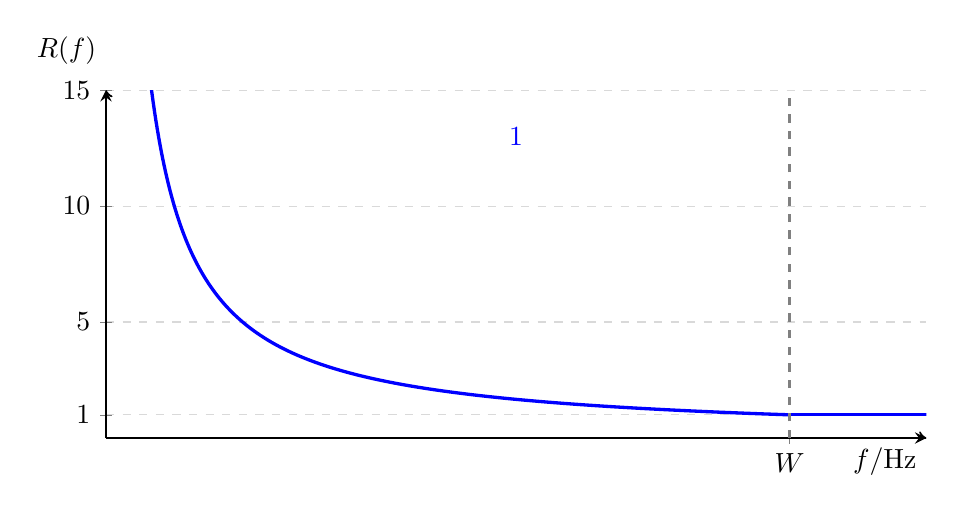
\begin{tikzpicture}
    \begin{axis}[
        width=12cm,
        height=6cm,
        xlabel={$f / \text{Hz}$},
        ylabel={$R(f)$},
        axis lines=middle,
        axis line style={thick},
        xmin=0, xmax=6000,
        ymin=0, ymax=15,
        xtick={0,5000},
        xticklabels={$0$, $W$},
        ytick={0,1,5,10,15},
        xlabel style={at={(ticklabel* cs:1)},anchor=north east},
        ylabel style={at={(ticklabel* cs:1)},anchor=north east,yshift=0.8cm},
        xmajorgrids=false,
        ymajorgrids=true,
        grid style={dashed,gray!30},
        samples=500,
    ]
    \addplot[very thick,blue,domain=100:5000] {5000/x};
    \addplot[very thick,blue,domain=5000:6000] {1};
    \draw[dashed,thick,gray] (axis cs:5000,0) -- (axis cs:5000,15);
    \node[blue] at (axis cs:3000,13) {$1$};
    \draw[thick,->] (axis cs:5800,0) -- (axis cs:6000,0);
    \draw[thick,->] (axis cs:0,14) -- (axis cs:0,15);
    \end{axis}
    \end{tikzpicture}
    \newline
    For 400 Hz, amplification needed = $\frac{1}{0.08}$ = 12.5
    \newline
    For 1000 Hz, amplification needed = $\frac{1}{0.2}$ = 5

    \section{Problem 2}
    \subsection{Part (a)}
    Two possible filter responses that satisfy the input-output relationship:
    
    \begin{figure}[h]
    \centering
    \begin{subfigure}{0.48\textwidth}
    \centering
    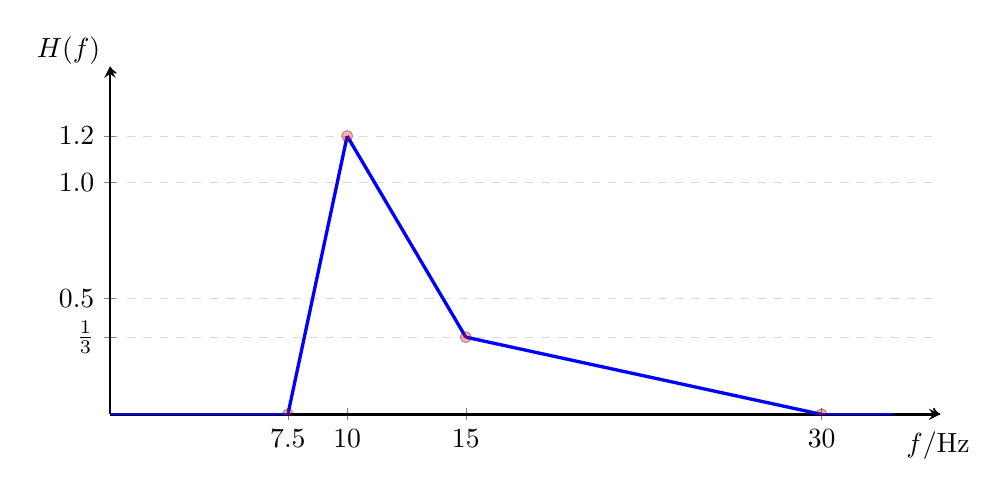
\begin{tikzpicture}
    \begin{axis}[
        width=\textwidth,
        height=6cm,
        xlabel={$f / \text{Hz}$},
        ylabel={$H(f)$},
        axis lines=middle,
        axis line style={thick},
        xmin=0, xmax=35,
        ymin=0, ymax=1.5,
        xtick={7.5,10,15,30},
        xticklabels={$7.5$, $10$, $15$, $30$},
        ytick={0,0.333,0.5,1.0,1.2},
        yticklabels={$0$, $\frac{1}{3}$, $0.5$, $1.0$, $1.2$},
        xlabel style={at={(ticklabel* cs:1)},anchor=north east,xshift=0.5cm, yshift=-0.1cm},
        ylabel style={at={(ticklabel* cs:1)},anchor=north east,yshift=0.5cm},
        xmajorgrids=false,
        ymajorgrids=true,
        grid style={dashed,gray!30},
        samples=500,
    ]
    \addplot[very thick,blue,domain=0:7.5] {0};
    \addplot[very thick,blue,domain=7.5:10] {1.2*(x-7.5)/2.5};
    \addplot[very thick,blue,domain=10:15] {1.2 - (1.2-0.333)*(x-10)/5};
    \addplot[very thick,blue,domain=15:30] {0.333*(30-x)/15};
    \addplot[very thick,blue,domain=30:35] {0};
    \draw[fill=red,opacity=0.3] (axis cs:7.5,0) circle (2pt);
    \draw[fill=red,opacity=0.3] (axis cs:10,1.2) circle (2pt);
    \draw[fill=red,opacity=0.3] (axis cs:15,0.333) circle (2pt);
    \draw[fill=red,opacity=0.3] (axis cs:30,0) circle (2pt);
    \draw[thick,->] (axis cs:33,0) -- (axis cs:35,0);
    \draw[thick,->] (axis cs:0,1.4) -- (axis cs:0,1.5);
    \end{axis}
    \end{tikzpicture}
    \caption{Filter Response 1}
    \end{subfigure}
    \hfill
    \begin{subfigure}{0.48\textwidth}
    \centering
    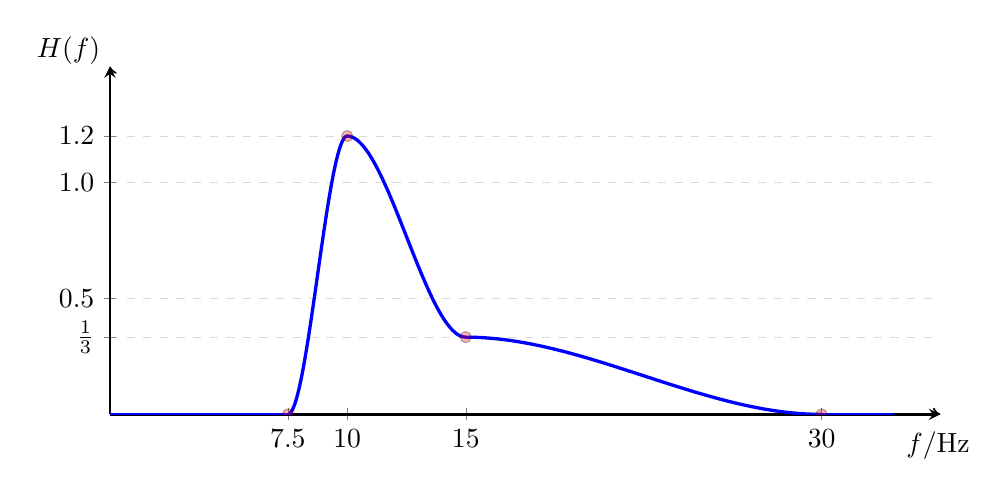
\begin{tikzpicture}
    \begin{axis}[
        width=\textwidth,
        height=6cm,
        xlabel={$f / \text{Hz}$},
        ylabel={$H(f)$},
        axis lines=middle,
        axis line style={thick},
        xmin=0, xmax=35,
        ymin=0, ymax=1.5,
        xtick={7.5,10,15,30},
        xticklabels={$7.5$, $10$, $15$, $30$},
        ytick={0,0.333,0.5,1.0,1.2},
        yticklabels={$0$, $\frac{1}{3}$, $0.5$, $1.0$, $1.2$},
        xlabel style={at={(ticklabel* cs:1)},anchor=north east,xshift=0.5cm, yshift=-0.1cm},
        ylabel style={at={(ticklabel* cs:1)},anchor=north east,yshift=0.5cm},
        xmajorgrids=false,
        ymajorgrids=true,
        grid style={dashed,gray!30},
        samples=500,
    ]
    \addplot[very thick,blue,domain=0:7.5,smooth] {0};
    \addplot[very thick,blue,domain=7.5:10,smooth] {1.2*((x-7.5)/2.5)^2*(3-2*(x-7.5)/2.5)};
    \addplot[very thick,blue,domain=10:15,smooth] {1.2 - (1.2-0.333)*((x-10)/5)^2*(3-2*(x-10)/5)};
    \addplot[very thick,blue,domain=15:30,smooth] {0.333*((30-x)/15)^2*(3-2*(30-x)/15)};
    \addplot[very thick,blue,domain=30:35,smooth] {0};
    \draw[fill=red,opacity=0.3] (axis cs:7.5,0) circle (2pt);
    \draw[fill=red,opacity=0.3] (axis cs:10,1.2) circle (2pt);
    \draw[fill=red,opacity=0.3] (axis cs:15,0.333) circle (2pt);
    \draw[fill=red,opacity=0.3] (axis cs:30,0) circle (2pt);
    \draw[thick,->] (axis cs:33,0) -- (axis cs:35,0);
    \draw[thick,->] (axis cs:0,1.4) -- (axis cs:0,1.5);
    \end{axis}
    \end{tikzpicture}
    \caption{Filter Response 2}
    \end{subfigure}
    \end{figure}
    \newpage
    \subsection{Part (b)}
    \[v(t) = w(t)\cos(120\pi t) = [2\sin(40\pi t) + \sin(20\pi t)]\cos(120\pi t)\]
    \[v(t) = 2\sin(40\pi t)\cos(120\pi t) + \sin(20\pi t)\cos(120\pi t)\]
    \[v(t) = \sin(160\pi t) - \sin(80\pi t) + \frac{1}{2}\sin(140\pi t) - \frac{1}{2}\sin(100\pi t)\]
    
    The frequency components of $v(t)$ are:
    \begin{itemize}
        \item $f = 40$ Hz: amplitude $|1| = 1$
        \item $f = 50$ Hz: amplitude $|-\frac{1}{2}| = 0.5$
        \item $f = 70$ Hz: amplitude $|\frac{1}{2}| = 0.5$
        \item $f = 80$ Hz: amplitude $|1| = 1$
    \end{itemize}
    \noindent The spectrum of $v(t)$ is as follows:
    
    \noindent
    \begin{tikzpicture}
    \begin{axis}[
        width=12cm,
        height=6cm,
        xlabel={$f / \text{Hz}$},
        ylabel={$V(f)$},
        axis lines=middle,
        axis line style={thick},
        xmin=0, xmax=90,
        ymin=0, ymax=1.5,
        xtick={40,50,70,80},
        xticklabels={$40$, $50$, $70$, $80$},
        ytick={0,0.5,1.0},
        xlabel style={at={(ticklabel* cs:1)},anchor=north east, xshift=0.3cm, yshift=-0.1cm},
        ylabel style={at={(ticklabel* cs:1)},anchor=north east, yshift=0.3cm},
        xmajorgrids=false,
        ymajorgrids=true,
        grid style={dashed,gray!30},
    ]
    \draw[very thick,blue,->] (axis cs:40,0) -- (axis cs:40,1) node[above] {$1$};
    \draw[very thick,red,->] (axis cs:50,0) -- (axis cs:50,0.5) node[above] {$0.5$};
    \draw[very thick,purple,->] (axis cs:70,0) -- (axis cs:70,0.5) node[above] {$0.5$};
    \draw[very thick,orange,->] (axis cs:80,0) -- (axis cs:80,1) node[above] {$1$};
    \draw[thick,->] (axis cs:85,0) -- (axis cs:90,0);
    \draw[thick,->] (axis cs:0,1.4) -- (axis cs:0,1.5);
    \end{axis}
    \end{tikzpicture}
    

    \section{Problem 3}
    \subsection{Part (a)}
    In this case, $f_{o}$ is the sampling frequency of $g(t)$.

    \subsection{Part (b)}
    Given $x(t) = \sum_{j=0}^{J} B_j \sin(2\pi j f_x t)$.
    The bandwidth of $x(t)$ is:
    \[ W = J f_x \]
    According to Nyquist sampling theorem,
    \[ f_0 \geq 2W = 2J f_x \]
    
    \noindent Therefore, a proper value for $f_0$ is:
    \[ f_0 = 2J f_x \]
    \newpage
    \subsection{Part (c)}
    Given $J = 3$, $B_{j} = 1 / (j+1)^2$, $A_{k} = 1$ for all $k$.
    \newline Calculating the amplitudes of $x(t)$:
    \newline$B_0 = \frac{1}{(0+1)^2} = 1 \quad$
    $B_1 = \frac{1}{(1+1)^2} = \frac{1}{4}$
    $B_2 = \frac{1}{(2+1)^2} = \frac{1}{9}$
    $B_3 = \frac{1}{(3+1)^2} = \frac{1}{16}$
    \newline Therefore, $x(t)$ has frequency components at:
    \begin{itemize}
        \item $f = 0$: sin(0) = 0
        \item $f = f_x$: amplitude $B_1 = 1/4$
        \item $f = 2f_x$: amplitude $B_2 = 1/9$
        \item $f = 3f_x$: amplitude $B_3 = 1/16$
    \end{itemize}

    \noindent bandwidth $W = 3f_x$. From Part (b), $f_0 = 2W = 6f_x$.

    \noindent Frequency-domain spectrum of $x(t)$ (one-sided):
    \newline
    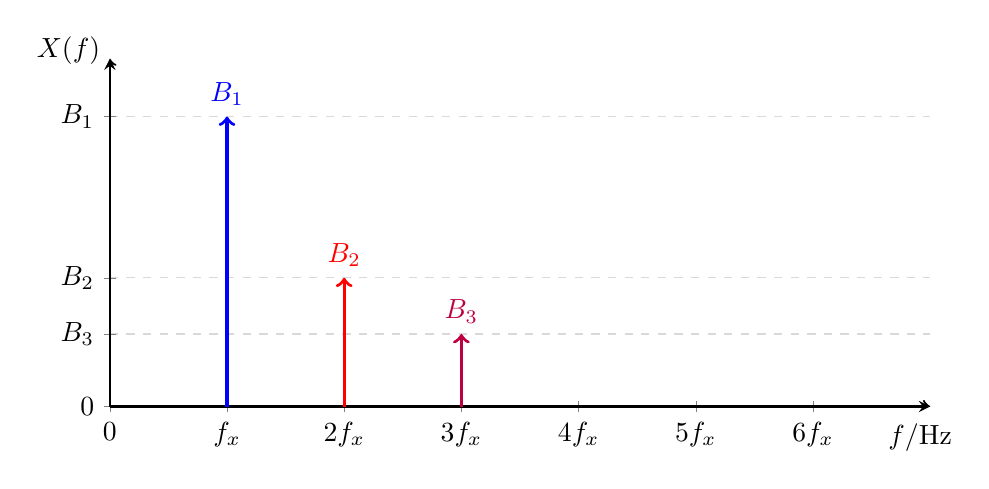
\begin{tikzpicture}
    \begin{axis}[
        width=12cm,
        height=6cm,
        xlabel={$f / \text{Hz}$},
        ylabel={$X(f)$},
        axis lines=left,
        axis line style={thick},
        xmin=0, xmax=7,
        ymin=0, ymax=0.6,
        xtick={0,1,2,3,4,5,6},
        xticklabels={$0$, $f_x$, $2f_x$, $3f_x$, $4f_x$, $5f_x$, $6f_x$},
        ytick={0,0.125,0.222,0.5},
        yticklabels={$0$, $B_3$, $B_2$, $B_1$},
        xlabel style={at={(ticklabel* cs:1)},anchor=north east, xshift=0.4cm, yshift=-0.1cm},
        ylabel style={at={(ticklabel* cs:1)},anchor=north east,rotate=-90, yshift=0.4cm},
        xmajorgrids=false,
        ymajorgrids=true,
        grid style={dashed,gray!30},
    ]
    \draw[very thick,blue,->] (axis cs:1,0) -- (axis cs:1,0.5) node[above] {$B_1$};
    \draw[very thick,red,->] (axis cs:2,0) -- (axis cs:2,0.222) node[above] {$B_2$};
    \draw[very thick,purple,->] (axis cs:3,0) -- (axis cs:3,0.125) node[above] {$B_3$};
    \draw[thick,->] (axis cs:6.5,0) -- (axis cs:7,0);
    \draw[thick,->] (axis cs:0,0.55) -- (axis cs:0,0.6);
    \end{axis}
    \end{tikzpicture}

    \noindent Frequency-domain spectrum of $s(t) = x(t) \cdot g(t)$ (one-sided):
    \newline
    \noindent (Note: The spectrum of $s(t)$ is a graph of x(t) repeated every $6f_x$, i.e. $f_0$.)
    \newline
    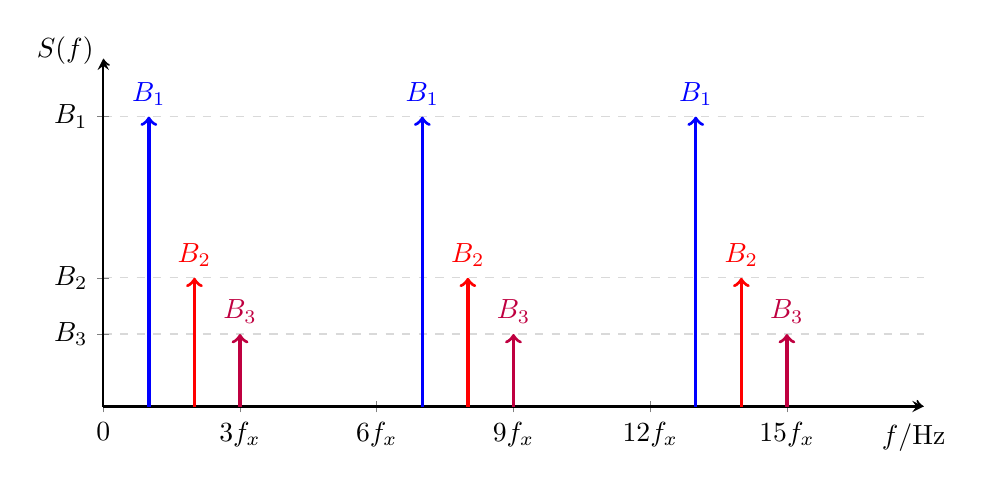
\begin{tikzpicture}
    \begin{axis}[
        width=12cm,
        height=6cm,
        xlabel={$f / \text{Hz}$},
        ylabel={$S(f)$},
        axis lines=left,
        axis line style={thick},
        xmin=0, xmax=18,
        ymin=0, ymax=0.6,
        xtick={0,3,6,9,12,15},
        xticklabels={$0$, $3f_x$, $6f_x$, $9f_x$, $12f_x$, $15f_x$},
        ytick={0.125,0.222,0.5},
        yticklabels={$B_3$, $B_2$, $B_1$},
        xlabel style={at={(ticklabel* cs:1)},anchor=north east, xshift=0.4cm, yshift=-0.1cm},
        ylabel style={at={(ticklabel* cs:1)},anchor=north east,rotate=-90, yshift=0.4cm},
        xmajorgrids=false,
        ymajorgrids=true,
        grid style={dashed,gray!30},
    ]
    % Baseband (k=0)
    \draw[very thick,blue,->] (axis cs:1,0) -- (axis cs:1,0.5) node[above] {$B_1$};
    \draw[very thick,red,->] (axis cs:2,0) -- (axis cs:2,0.222) node[above] {$B_2$};
    \draw[very thick,purple,->] (axis cs:3,0) -- (axis cs:3,0.125) node[above] {$B_3$};
    % Replicas at f_0 (k=1) - f_0 = 6f_x
    \draw[very thick,blue,->] (axis cs:7,0) -- (axis cs:7,0.5) node[above] {$B_1$};
    \draw[very thick,red,->] (axis cs:8,0) -- (axis cs:8,0.222) node[above] {$B_2$};
    \draw[very thick,purple,->] (axis cs:9,0) -- (axis cs:9,0.125) node[above] {$B_3$};
    % Replicas at 2f_0 (k=2) - 2f_0 = 12f_x
    \draw[very thick,blue,->] (axis cs:13,0) -- (axis cs:13,0.5) node[above] {$B_1$};
    \draw[very thick,red,->] (axis cs:14,0) -- (axis cs:14,0.222) node[above] {$B_2$};
    \draw[very thick,purple,->] (axis cs:15,0) -- (axis cs:15,0.125) node[above] {$B_3$};
    \draw[thick,->] (axis cs:17.5,0) -- (axis cs:18,0);
    \draw[thick,->] (axis cs:0,0.55) -- (axis cs:0,0.6);
    \end{axis}
    \end{tikzpicture}

    \newpage
    \noindent Ideal low-pass filter $R(f)$ to recover $x(t)$ from $s(t)$:
    \newline
    \begin{tikzpicture}
    \begin{axis}[
        width=12cm,
        height=6cm,
        xlabel={$f / \text{Hz}$},
        ylabel={$R(f)$},
        axis lines=left,
        axis line style={thick},
        xmin=0, xmax=7,
        ymin=0, ymax=1.2,
        xtick={0,3,6},
        xticklabels={$0$, $3f_x$, $6f_x$},
        ytick={0,1},
        xlabel style={at={(ticklabel* cs:1)},anchor=north east},
        ylabel style={at={(ticklabel* cs:1)},anchor=north east,rotate=-90},
        xmajorgrids=false,
        ymajorgrids=true,
        grid style={dashed,gray!30},
        samples=500,
    ]
    \addplot[very thick,blue,domain=0:3] {1};
    \addplot[very thick,blue,domain=3:9] {0};
    \draw[dashed,thick,gray] (axis cs:3,0) -- (axis cs:3,1);
    \draw[thick,->] (axis cs:6.5,0) -- (axis cs:7,0);
    \draw[thick,->] (axis cs:0,1.1) -- (axis cs:0,1.2);
    \end{axis}
    \end{tikzpicture}

    \noindent The filter passes frequencies from $0$ to $3f_x$ (the base bandwidth) and rejects all replicas at higher frequencies.
    

    \section{Problem 4}
    \subsection{Part (a)}
    For $m(t)$, bandwidth $W = 50$Hz. Thus, the Nyquist rate $f_{s} = 2W$ = 100Hz.
    \subsection{Part (b)}
    Dynamic range = $\frac{A_{max}}{A_{min}} = \frac{1.7}{0.3} = 5.67$
    \newline $m(t)$ spanning [-3, 3].
    
    \subsection{Part (c)}
    Since range of sin function = [-1, 1], the range of $m(t)$ = [-3, 3].
    \newline 
    We can see when $m(t)$ = -2 or 0 or 2, the error is the largest because they are in the middle of the quantization levels.
    \newline i.e. largest quantization error = 0.5
    \subsection{Part (d)}
    Assuming $f_{o}$ = 100Hz, sample period = 0.01s.
    \newline
    For $t = 1.02$, $m(t) \approx 0.898$ 
    For $t = 1.03$, $m(t) \approx -0.765$
    For $t = 1.04$, $m(t) \approx 0.575$
    For $t = 1.05$, $m(t) \approx 2.569$ 
    Quantized value = [1, -1, 1, 3]
    \subsection{Part (e)}
    4-level quantizer: 2 bit per sample, 100 samples per second.
    \newline
    Total bits needed = $2 * 100 * 45 = 9000$bits
    \section{Problem 5}
    \subsection{Part (a)}
    Value $0$: $17$ times, Value $50$: $8$ times.

    \noindent Histogram:
    \newline
    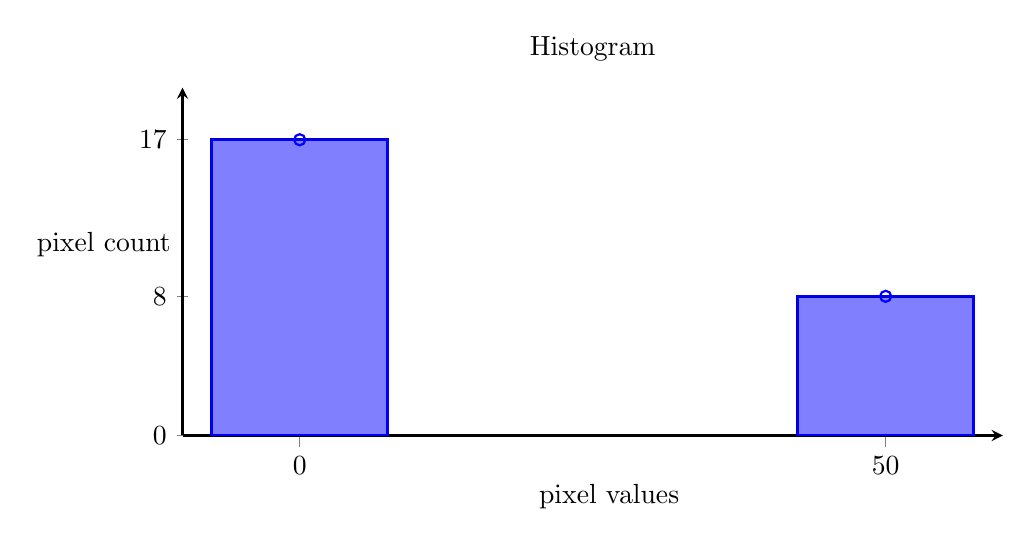
\begin{tikzpicture}
    \begin{axis}[
        width=12cm,
        height=6cm,
        title={Histogram},
        xlabel={pixel values},
        ylabel={pixel count},
        axis lines=left,
        axis line style={thick},
        xmin=-10, xmax=60,
        ymin=0, ymax=20,
        xtick={0,50},
        xticklabels={$0$, $50$},
        ytick={0,8,17},
        yticklabels={$0$, $8$, $17$},
        xlabel style={at={(ticklabel* cs:1)},anchor=north,yshift=-0.5cm, xshift=-5cm},
        ylabel style={at={(ticklabel* cs:1)},anchor=center,yshift=1cm, xshift=-2cm,rotate=-90},
        xmajorgrids=false,
        ymajorgrids=false,
        ybar,
        bar width=15,
        bar shift=0,
    ]
    \addplot[fill=blue!50,draw=blue!70!black,very thick] coordinates {
        (0,17)
        (50,8)
    };
    \addplot[blue, thick, mark=o, mark options={fill=white, draw=blue, thick}, only marks] coordinates {(0,17) (50,8)};
    \addplot[blue, thick, no markers] coordinates {(0,17) (50,8)};
    \end{axis}
    \end{tikzpicture}
    
    \subsection{Part (aii)}
    $G = \frac{1}{11}\begin{bmatrix}
        50 & 150 & 150 & 100 & 0 \\
        50 & 300 & 350 & 400 & 100 \\
        100 & 400 & 350 & 350 & 150 \\
        50 & 200 & 400 & 300 & 150 \\
        50 & 50 & 100 & 50 & 50 \\
    \end{bmatrix} \approx \begin{bmatrix}
        4.545 & 13.64 & 13.64 & 9.091 & 0 \\
        4.545 & 27.27 & 31.82 & 36.36 & 9.091 \\
        9.091 & 36.36 & 31.82 & 31.82 & 13.64 \\
        4.545 & 18.18 & 36.36 & 27.27 & 13.64 \\
        4.545 & 4.545 & 9.091 & 4.55 & 4.545 \\
    \end{bmatrix}$

    \subsection{Part (bi)}
    By observation, most values in $I$ is between 90 and 100. However, in $I[2,2]$ and $I[4,4]$ the values are either larger or smaller than this range for a huge difference.
    
    \noindent Therefore, if we perform median filtering, the values of $I[2,2]$ and $I[4,4]$ will be replaced by the median of the surrounding values.
    the sharp edge will be blurred.
    
    \subsection{Part (bii)}
    $J = \begin{bmatrix}
        0 & 98 & 98 & 97 & 0 \\
        98 & 98 & 98 & 98 & 96 \\
        96 & 98 & 98 & 97 & 94 \\
        95 & 97 & 96 & 97 & 50 \\
        0 & 95 & 50 & 50 & 0
    \end{bmatrix}$

    \subsection{Part (biii)}
    for $n \times n$ median filtering with zero padding, the data in he corner will be replaced by zero.
    \newline Also, border pixels will be biased towards zero.
\end{document}